\documentclass[a4paper,10pt]{article}

\usepackage{graphicx} % Required for inserting images
\usepackage[left=2.5cm, right=2.5cm, top=3cm, bottom=3cm]{geometry}

\usepackage[UTF8]{ctex} % 引入中文宏包
\usepackage{amsmath} 
% 引入表格美化包（三线表）
\usepackage{booktabs}
% 引入图片插入包
\usepackage{graphicx}
% 引入浮动体控制包（用于固定表格/图片位置）
\usepackage{float}
% 引入超链接包（可选）
\usepackage{hyperref}

\usepackage{listings}
\usepackage{xcolor}

% 表格美化包 (用于粗横线 \toprule, \bottomrule)
\usepackage{booktabs}

% 数组包 (用于定义列格式)
\usepackage{array}

% 设置代码块样式
\lstset{
    language=Python,
    basicstyle=\ttfamily\footnotesize, % 字体大小
    keywordstyle=\color{blue},         % 关键字颜色
    stringstyle=\color{red},           % 字符串颜色
    commentstyle=\color{green!50!black}, % 注释颜色
    numbers=left,                      % 行号显示在左侧
    numberstyle=\tiny\color{gray},     % 行号样式
    stepnumber=1,                      % 行号间隔
    breaklines=true,                   % 自动换行
    frame=single,                      % 代码框
    backgroundcolor=\color{gray!5},    % 背景色
    showstringspaces=false,            % 不显示字符串中的空格标记
    captionpos=b,                      % 标题位置
    tabsize=4                          % 制表符宽度
}



\begin{document}

\begin{center}
    % --- 标题部分 ---
    \vspace*{1cm}
    {\Huge ZO-1 Capstone 双周报 1}
    
    \vspace{2.5cm}
    
    % --- 日期部分 ---
    {\Large January 25, 2026}
    
    \vspace{1.5cm}
    
    % --- 表格部分 ---
    % 设置行高为1.5倍，增加行间距以匹配图片
    \renewcommand{\arraystretch}{1.5}
    
    % 定义表格：两列
    % >{\bfseries}l 表示第一列左对齐且自动加粗
    % l 表示第二列左对齐
    % @{} 用于去除表格左右两侧的默认留白，使横线与文本对齐
    \begin{tabular}{@{} >{\bfseries}l l @{}}
    
        \toprule[1.5pt] % 顶部粗横线
        
        项目企业 & 中欧瑞博 \\
        
        项目名称 & 股东回报因子探索：考虑净回购的股息率 + 因子 \\
        
        % 这里替换为你要求的内容，并格式化了学号的括号以匹配原图风格
        学生姓名 & 沈可涵 (123090483), 蒋之伟 (123090233), Yantao Yang (123090731) \\
        
        报告周期 & 2026 年 1 月 5 日至 2026 年 1 月 25 日 \\
        
        提交日期 & 2026 年 1 月 25 日 \\
        
        \bottomrule[1.5pt] % 底部粗横线
        
    \end{tabular}
\end{center}



\section{大纲}

本文围绕“考虑净回购的股息率+（Shareholder Return / Total Payout）因子”在港股通样本中的数据工程与可行性验证展开，全文结构如下：

\begin{enumerate}
    \item \textbf{文献调研进展（第 2 节）}\\
    梳理总派现（分红+回购）视角的资产定价研究、股息率 plus / 股东回报率因子框架，以及周期调整指标（如 CATY）等文献脉络，并总结对港股回购变量构建的启示。

    \item \textbf{数据挖掘与样本构建（第 3 节）}\\
    介绍港股通名单数据与港股公告数据两类源数据；说明公告样本与港股通成分股的同日匹配方法；基于标题关键词识别回购公告，并按季度统计回购公告数量以刻画时间分布特征（包含趋势折线图与解读）。

    \item \textbf{回购公告正文获取与结构化处理（第 4 节）}\\
    在标题级识别基础上，进一步下载回购公告 PDF 正文并解析文本；构建逐步筛选流程（初筛、去噪、可获取性筛选）；通过正则抽取回购股份数量、价格与金额等字段，并对回购公告进行类型细分（执行类/授权类/其他），为后续回购强度度量提供结构化数据基础。

    \item \textbf{关键挑战与方法论考量（第 5 节）}\\
    讨论两类核心问题：公告表述异质性与重复披露导致的噪声与去重困难；回购事件低频属性与日频因子研究之间的频率不匹配，并分析其对变量定义、聚合窗口与信息衰减机制设计的影响。

    \item \textbf{初步解决方案设想（第 6 节）}\\
    提出从公告到“回购行为”信号的转化思路：类型区分、聚合规则弱化重复披露影响；引入正文信息提升识别精度；并给出低频事件映射为日频变量的统一框架（事件虚拟变量、滚动窗口累积、记忆衰减型指标），作为后续因子构建与实证比较的起点。

    \item \textbf{附录（Appendix）}\\
    附录 A 给出文献综述的扩展版本（含公式与关键结论）；附录 B 汇总公告正文下载、文本解析与字段抽取的核心代码，以便复现与后续迭代。
\end{enumerate}


\section{文献调研进展}

\subsection{核心文献梳理}

本阶段重点阅读并整理了三类具有代表性的研究（详细内容见附录\ref{sec:appendix_literature}）：

\begin{enumerate}
    \item \textbf{总回报（Dividends + Buybacks）资产定价模型}
    \begin{itemize}
        \item 文献指出，长期股票收益可以主要由\textbf{总派现（Total Payout）} 解释，而非仅由分红驱动；
        \item 在考虑回购后的情形下，传统股息贴现模型（DDM）对未来收益存在系统性低估。
    \end{itemize}

    \item \textbf{股息率 Plus / 净回购因子研究}
    \begin{itemize}
        \item 相关研究将净回购规模（回购 $-$ 增发）标准化后，与股息率合并构建“股息率 plus”指标；
        \item 实证结果显示，该类因子在预测长期收益、解释价值溢价方面具有更强稳定性。
    \end{itemize}

    \item \textbf{周期调整与宏观一致性}
    \begin{itemize}
        \item 总回报收益率在周期调整后（如 CATY）对预期收益的解释能力不弱于 CAPE 等经典估值指标；
        \item 聚合层面的总派现增长与 GDP 增长具有较强一致性。
    \end{itemize}
\end{enumerate}

\subsection{文献结论的研究启示}

\begin{itemize}
    \item 回购并非分红的简单替代，而是影响股价的重要现金分配渠道；
    \item 将回购忽略可能导致对企业估值与预期收益的系统性偏误；
    \item 需要在微观层面准确识别回购行为，在宏观与横截面层面进行规范化处理。
\end{itemize}








\section{数据挖掘与样本构建}

\subsection{数据来源}

本文使用两类港股层面的原始数据：

\begin{enumerate}
    \item \textbf{港股通股票名单数据（HSCI.csv）}\\
    该数据记录各交易日纳入港股通机制的股票名单，用于刻画研究样本的可投资范围。
    
    \item \textbf{港股上市公司公告数据（hk\_announcement.csv）}\\
    该数据包含港股上市公司公告披露信息，用于识别回购相关的信息披露事件。
\end{enumerate}

为明确数据覆盖范围与规模，表 \ref{tab:data_overview} 汇总了两类源数据的时间范围、股票覆盖与记录条数，并进一步给出“港股通$\times$公告”同日匹配后的样本规模。

% 表 1 数据集概览
\begin{table}[H]
    \centering
    \caption{数据集概览（Data Overview）}
    \label{tab:data_overview}
    \resizebox{\textwidth}{!}{% 自动缩放表格以适应页面宽度
    \begin{tabular}{llrrp{6cm}} % p{6cm}用于控制备注列宽度并允许自动换行
        \toprule
        \textbf{数据集} & \textbf{时间范围} & \textbf{股票数量} & \textbf{记录条数} & \textbf{备注} \\
         & & \footnotesize{(去重 order\_book\_id)} & & \\
        \midrule
        港股通名单（HSCI） & 2005-01-03 $\sim$ 2025-12-31 & 1,126 & 2,019,624 & date$\times$sid \\
        港股公告（Announcement） & 2014-08-01 $\sim$ 2025-09-30 & 1,081 & 1,305,817 & 全量公告 \\
        港股通$\times$公告（Join 后样本） & 2014-08-01 $\sim$ 2025-09-30 & 987 & 790,869 & inner join on (info\_date, order\_book\_id) \\
        \bottomrule
    \end{tabular}
    }
    \vspace{0.2cm} % 表格与表注之间的间距
    \begin{flushleft}
        \footnotesize
        \textbf{注：}股票数量按 \texttt{order\_book\_id} 去重口径统计；“Join 后样本”为公告在披露日属于港股通成分股的公告集合。
    \end{flushleft}
\end{table}

\subsection{样本对齐与筛选}

为保证研究样本具有明确的可交易边界并避免前视偏差，本文采用“同日匹配”的方式将公告与港股通成分股名单进行对齐：仅保留公告披露日（\texttt{info\_date}）公司仍属于港股通成分股（\texttt{order\_book\_id}）的公告记录。表 \ref{tab:filtering} 展示了样本筛选前后公告数量及股票覆盖的变化。

% 表 2 样本筛选过程
\begin{table}[H]
    \centering
    \caption{样本筛选过程与样本量变化（Filtering Pipeline）}
    \label{tab:filtering}
    \begin{tabular}{lrr}
        \toprule
        \textbf{筛选步骤} & \textbf{剩余公告数} & \textbf{剩余股票数} \\
        \midrule
        原始公告数据 & 1,305,817 & 1,081 \\
        匹配港股通当日成分股（同日 inner join） & 790,869 & 987 \\
        \bottomrule
    \end{tabular}
    \vspace{0.2cm}
    \begin{flushleft}
        \footnotesize
        \textbf{注：}同日匹配指在 \texttt{(info\_date, order\_book\_id)} 维度进行 inner join；筛选后样本更贴近港股通可投资集合。
    \end{flushleft}
\end{table}

\subsection{回购公告的识别与提取}

在“港股通$\times$公告”的有效样本中，本文进一步聚焦\textbf{股份回购相关公告}。具体做法为：基于公告标题字段进行关键词匹配，识别包含“回购/购回/buyback/repurchase”等表述的公告，从而形成回购公告子样本，用于后续统计分析与因子构造。

\subsection{回购公告的时间分布特征}

在识别出回购公告后，本文对其时间分布特征进行整理，重点观察回购公告在样本期内的动态变化，并按季度统计回购公告数量（及可选地统计涉及回购的公司数），以刻画市场回购行为的周期性与阶段性特征。







% --- 插入折线图位置 ---
% 请将 'your_figure_filename.png' 替换为你本地折线图的文件名
\begin{figure}[H] 
    \centering
    % 如果图片太宽，可以使用 [width=\textwidth]
    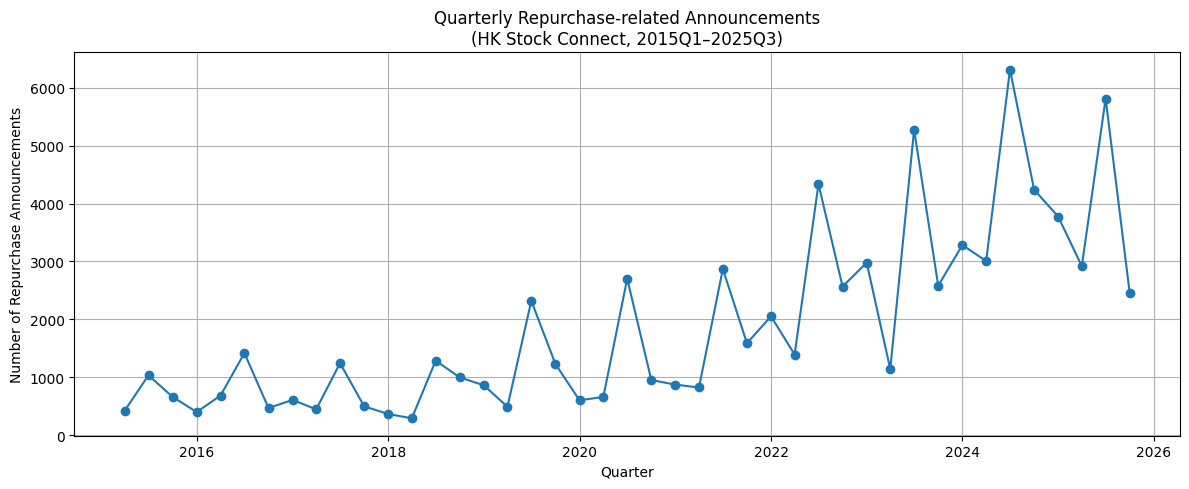
\includegraphics[width=0.9\textwidth]{image.png} 
    
    % 此处使用 demo 占位符，实际使用时请取消上面一行的注释并删除下面一行
    % \fbox{\parbox[c][6cm]{0.8\textwidth}{\centering 图片占位符：请在此处插入你的季度回购公告趋势折线图}}
    
    \caption{港股通公司回购公告的季度分布（2015Q1--2025Q3）}
    \label{fig:buyback_trend}
    \vspace{0.2cm}
    \begin{flushleft}
        \footnotesize
        \textbf{说明：}横轴为季度；纵轴为回购公告数量（及可选的回购公司数）。
    \end{flushleft}
\end{figure}

% --- 新增的图表分析文字 ---

图 \ref{fig:buyback_trend} 展示了 2015 年第一季度至 2025 年第三季度期间，港股通成分股中回购相关公告的季度数量变化。从整体趋势来看，回购公告数量呈现出显著的阶段性上升特征，并伴随一定的周期性波动。

首先，在 2015Q1--2018Q4 阶段，回购公告数量整体处于较低水平，季度公告数大多在 1,500 条以下，波动幅度相对有限，表明港股通公司在该阶段的股份回购行为较为谨慎，回购并未成为常态化的资本配置手段。

进入 2019 年之后，回购公告数量开始明显抬升。尤其在 2019Q3、2020Q2 及 2021Q2 等时间点，季度回购公告数出现阶段性跃升，显示在市场环境发生变化时，上市公司更频繁地通过回购向市场释放估值与信号信息。

自 2022 年起，回购公告数量进一步进入高位区间。多个季度的回购公告数显著超过 3,000 条，并在 2024 年前后达到样本期内的峰值水平（超过 6,000 条）。这一现象表明，回购已逐步成为港股通公司中较为普遍的股东回报与资本管理工具，而非偶发性行为。

此外，图 \ref{fig:buyback_trend} 还显示出一定的短期波动与集中爆发特征：部分季度回购公告数量快速上升后在下一季度出现回落，反映回购行为在执行节奏上仍受到市场情绪、股价波动及公司内部决策周期等因素的共同影响。

总体而言，图 \ref{fig:buyback_trend} 所揭示的时间分布特征表明，港股通公司回购行为在样本期内经历了从“低频试探”到“高频常态化”的演进过程。这一趋势为后续基于回购公告构建特征变量、并检验其资产定价含义提供了重要的时间维度依据。


\section{回购公告正文的获取与结构化处理}

在前文中，本文已基于公告标题与港股通成分信息，构建了回购相关公告的基础样本，并分析了其时间分布特征。然而，仅依赖公告标题进行识别，仍可能混入大量\textbf{非实际回购执行}的公告类型（如回购授权、股东大会通函等），同时也无法获取回购规模、价格与金额等关键信息。因此，本文进一步对回购公告进行\textbf{正文级别的数据获取与结构化处理}，以支持后续更精细的回购行为度量。（详细内容见附录\ref{sec:appendix:code_buyback}）

\subsection{回购公告样本的逐步筛选}

基于港股公告全量数据，本文采用“\textbf{由宽到严}”的多阶段筛选策略构建回购公告候选集：

\begin{enumerate}
    \item \textbf{关键词初筛（标题级）}
    
    首先基于中英文回购关键词（如“股份回购”、“购回”、“buyback”、“repurchase”等），在公告标题中进行匹配，得到初始回购相关公告 \textbf{49,687 条}。

    \item \textbf{类别过滤与噪声剔除}
    
    为减少非回购执行类公告的干扰，进一步限定公告所属类别为 \textit{Announcements and Notices} 或 \textit{Circulars}，并显式排除与股东大会、年会通函及一般性授权相关的公告。经该步骤后，回购公告样本数量缩减至 \textbf{10,144 条}。

    \item \textbf{正文可获取性筛选}
    
    在上述样本中，仅保留包含有效公告链接（PDF）的记录，以保证后续正文解析的可行性，最终得到 \textbf{3,332 条}可爬取的回购公告。
\end{enumerate}

该逐层筛选过程在保证样本相关性的同时，最大限度地降低了误识别与噪声引入的风险。

\subsection{回购公告正文的自动化下载}

针对筛选后的回购公告样本，本文设计并实现了一套\textbf{自动化公告爬取与文本解析流程}，主要特征包括：

\begin{itemize}
    \item \textbf{批量下载}：基于公告链接自动下载 PDF 文件；
    \item \textbf{断点续爬机制}：通过记录已完成索引与中间结果，支持程序中断后继续运行，确保大规模抓取过程的稳定性；
    \item \textbf{请求频率控制}：在爬取过程中设置延时机制，以避免对公告源网站造成过高访问压力。
\end{itemize}

在实际运行中，共尝试下载 \textbf{3,332 条}公告，其中 \textbf{3,177 条成功完成下载与文本解析}，整体成功率约为 \textbf{95\%}。未成功解析的公告主要由于 PDF 编码异常或文本不可提取所致。

\subsection{公告正文的文本解析与信息抽取}

在成功下载的公告 PDF 基础上，本文进一步对公告正文进行文本化处理，并尝试抽取与回购执行直接相关的关键信息，主要包括：

\begin{itemize}
    \item \textbf{回购股份数量}（Number of shares repurchased）
    \item \textbf{回购价格或价格区间}（Repurchase price）
    \item \textbf{回购总金额}（Aggregate consideration）
\end{itemize}

具体而言，本文基于正则表达式匹配中英文常见表述，对公告正文进行扫描，并为每一条公告记录是否成功识别上述信息。同时，保留文本长度与字段存在性标记，以衡量信息完整程度。

该结构化处理使得原本非结构化的公告文本被转化为可用于横截面与时间序列分析的量化变量，为后续构建回购强度、规模及执行节奏等指标提供了数据基础。

\subsection{回购公告类型的细分}

结合公告标题与正文内容，本文进一步对回购公告进行类型划分，主要包括：

\begin{itemize}
    \item \textbf{实际回购执行公告}（如每日回购披露）
    \item \textbf{回购授权类公告}（如一般性授权或授权更新）
    \item \textbf{其他回购相关公告}
\end{itemize}

该分类有助于在后续实证分析中区分“\textbf{意向性回购信息}”与“\textbf{已发生的回购行为}”，避免将授权公告与真实回购执行混合处理，从而提高回购变量的经济含义一致性。

\subsection{小结}

通过对回购公告正文的系统性下载与结构化处理，本文在标题级别识别的基础上，进一步构建了一个\textbf{正文可读、信息可量化、类型可区分}的回购公告数据库。该数据库不仅显著降低了噪声公告的干扰，也为后续回购强度指标构造及其市场效应分析奠定了坚实的数据基础。


\section{当前存在的问题与阻碍——数据处理中的关键挑战与方法论考量}

在基于港股公告构建回购相关变量的过程中，本文在数据获取与变量构造阶段面临若干具有代表性的现实挑战。本节对其中两项核心问题进行系统梳理，并讨论其对因子构建与实证分析的影响。

\subsection{回购公告表述异质性与重复披露问题}

\subsubsection{公告表述的非标准化特征}

港股市场中，上市公司在披露回购相关信息时并不存在统一的文本模板或披露格式。即使针对同一类回购行为，不同公司在公告标题及正文中的表述方式也存在显著差异，例如：

\begin{itemize}
    \item 中英文混合使用（“股份回购”、“购回股份”、“share buyback”、“repurchase”等）；
    \item 不同语义层级的披露（回购授权、回购执行、翌日披露、完成回购等）；
    \item 标题与正文信息不一致或信息粒度不对称。
\end{itemize}

这种表述异质性使得仅依赖公告标题或单一关键词进行识别，容易引入噪声或遗漏有效信息。

\subsubsection{单一回购事件的多次公告披露}

除表述差异外，港股回购公告还存在显著的\textbf{重复披露特征}。对于同一回购计划或回购授权，上市公司可能在不同时间点多次发布公告，例如：

\begin{itemize}
    \item 授权类公告（如一般性回购授权）；
    \item 每日或阶段性回购执行披露；
    \item 回购完成或进度更新公告。
\end{itemize}

因此，在公告层面观察到的“多条回购公告”并不必然对应多个独立的回购事件。若直接将公告条数视为回购强度，可能会高估回购行为的频率或规模。

\subsubsection{对变量构造的影响}

上述问题对回购变量构造提出了明确要求：

\begin{itemize}
    \item 需要区分“\textbf{意向性披露}”与“\textbf{实际回购执行}”；
    \item 需要在公告层面进行去重、聚合或类型区分，而非简单计数；
    \item 有必要在正文级别识别回购执行信息，以提高变量的经济含义一致性。
\end{itemize}

这也是本文进一步引入公告正文解析与回购类型细分的重要动机。

\subsection{低频事件数据与日频因子构建的张力}

\subsubsection{回购公告的天然低频属性}

从时间维度来看，回购公告属于典型的\textbf{低频公司事件数据}。即使在回购较为活跃的阶段，单个公司在较长时间窗口内发布回购公告的次数仍然有限，且公告发布时间在交易日之间高度不均匀。

然而，后续资产定价与因子分析通常依赖\textbf{日频或更高频率的数据结构}。这在事件数据与因子研究之间形成了天然的频率不匹配问题。

\subsubsection{从事件到日频的映射问题}

将低频回购事件转化为日频变量，需要解决以下关键问题：

\begin{itemize}
    \item \textbf{事件影响的持续时间}：回购公告是否仅在披露当日产生影响，或具有跨日效应；
    \item \textbf{多次公告的合并方式}：同一时间窗口内多条回购公告应如何聚合；
    \item \textbf{信息衰减与记忆机制}：回购信息对市场的影响是否随时间递减。
\end{itemize}

不同处理方式将直接影响日频因子的平滑程度、噪声水平及经济含义。

\subsubsection{方法论上的权衡}

在实际操作中，本文需要在以下维度进行权衡：

\begin{itemize}
    \item 采用\textbf{事件发生日虚拟变量（event dummy）}、\textbf{滚动窗口累积指标}，或\textbf{指数加权记忆型变量}；
    \item 在保持日频数据结构的同时，避免引入过度人为平滑；
    \item 确保构建的日频因子能够真实反映回购信息的时间分布与经济逻辑。
\end{itemize}

因此，低频事件到日频因子的映射并非简单的技术问题，而是因子经济含义与实证可解释性之间的综合取舍。

\subsection{小结}

总体而言，回购公告在文本表述与时间分布上的复杂性，使得其数据处理与因子构建显著不同于传统的高频价格或财务数据。本文通过引入公告正文解析、回购类型区分以及事件到日频的映射机制，力图在降低噪声的同时保留回购行为的核心信息，为后续日频回购因子的构建与检验提供稳健的数据基础。




\section{问题的初步解决方案设想}

针对前文所述回购公告在文本表述、披露频率及时间结构上的复杂性，本文在数据处理与变量构造阶段提出一套初步的解决方案。该方案的目标并非在一开始即给出最终形式的回购因子，而是在保证经济含义合理性的前提下，逐步将非结构化、低频的公告事件转化为可用于日频实证分析的数据结构。

\subsection{回购公告异质性与重复披露的处理思路}

\subsubsection{从“公告条数”到“回购行为”的转化}

鉴于同一回购行为可能对应多次公告披露，本文不直接将公告数量等同于回购强度，而是将“公告”视为对潜在回购行为的不同层级刻画。具体而言，初步解决方案包括：

\begin{itemize}
    \item \textbf{区分公告类型}：基于公告标题与正文内容，将回购相关公告划分为授权类公告、执行类公告及其他回购相关公告，避免将授权性披露与实际回购执行混合处理。
    \item \textbf{弱化重复披露的影响}：在后续变量构造中，不以同一公司在短期内的公告条数简单累加，而是通过聚合规则（如同一窗口内取最大值或是否发生）降低重复披露对回购强度度量的干扰。
\end{itemize}

该处理思路有助于将公告层面的噪声转化为更接近真实经济行为的信号。

\subsection{利用公告正文信息提升回购识别精度}

针对公告标题表述不统一的问题，本文引入公告正文层面的信息作为辅助判别依据。具体包括：

\begin{itemize}
    \item \textbf{正文级回购信息抽取}：通过对公告 PDF 正文进行文本解析，尝试识别回购股份数量、回购价格及回购金额等关键要素，以判断公告是否对应真实的回购执行行为。
    \item \textbf{基于正文的回购类型纠正}：若公告标题存在歧义，但正文中明确出现回购执行相关表述（如已回购股份数量），则将该公告重新归类为执行型回购公告。
\end{itemize}

通过引入正文信息，本文在一定程度上缓解了公告表述异质性带来的误识别问题，提高了回购事件识别的准确性。

\subsection{从低频回购事件到日频变量的映射框架}

\subsubsection{基本映射原则}

面对回购公告天然低频的特征，本文采用“事件驱动到时间序列”的映射思路，将回购公告转化为日频变量。初步遵循以下原则：

\begin{itemize}
    \item 回购信息在披露当日具有最强的信息含量；
    \item 回购公告可能对随后若干交易日产生持续影响；
    \item 同一时间窗口内多次公告应进行聚合处理。
\end{itemize}

\subsubsection{初步日频构造方式}

在方法设计阶段，本文考虑以下几种可行的日频映射方案，供后续实证比较：

\begin{itemize}
    \item \textbf{事件虚拟变量（Event Dummy）}：在公告披露当日设置回购事件指示变量，用于刻画回购信息的即时效应。
    \item \textbf{滚动窗口累积指标}：在固定时间窗口内（如过去 N 个交易日），累积或计数回购相关公告，以反映回购信息的短期集中程度。
    \item \textbf{记忆衰减型指标}：对回购事件赋予随时间递减的权重，使较近的回购公告对当前日的影响更大，从而刻画回购信息的持续性。
\end{itemize}

上述方法为低频事件向日频因子转化提供了统一的框架基础。

\subsection{方案的阶段性定位与后续扩展}

需要强调的是，本节提出的解决方案属于初步方法设计，其目的在于搭建从公告数据到因子构造的可行路径，而非直接给出最终最优因子形式。后续研究将基于该框架：

\begin{itemize}
    \item 对不同回购类型（授权型与执行型）分别构造日频变量；
    \item 比较不同时间映射方式在实证结果中的表现差异；
    \item 在控制其他公司特征后，检验回购因子的资产定价含义。
\end{itemize}






\appendix 

\label{sec:appendix_literature}
\section{文献综述：考虑股票回购的“股息率+”股东回报因子研究} \label{sec:appendix_literature}


\subsection{基于总派现率（Total Payout Yield）的资产定价研究}

传统资产定价与估值文献通常以股息率（Dividend Yield）作为刻画股票预期回报的重要状态变量，并据此检验长期回报的可预测性。然而，该类研究隐含假设企业主要通过现金分红向股东返还资本。随着股票回购在企业派现政策中的占比持续上升，仅使用股息率衡量股东回报将产生系统性测量误差。

在此背景下，Boudoukh et al. (2007) 提出以\textbf{总派现率（Total Payout Yield）}替代传统股息率，用以完整刻画企业向股东返还的现金流。作者将股东派现定义为现金分红与股票回购之和：

\begin{equation}
    \text{Total Payout}_t = D_t + B_t
\end{equation}

其中 $D_t$ 表示现金分红，$B_t$ 表示股票回购规模。相应地，总派现率定义为：

\begin{equation}
    \text{Total Payout Yield}_t = \frac{D_t + B_t}{P_t}
\end{equation}

其中 $P_t$ 为股票价格或市值。

在实证设定上，作者将传统的回报预测模型：

\begin{equation}
    R_{t+1} = \alpha + \beta \cdot DY_t + \varepsilon_{t+1}
\end{equation}

扩展为以总派现率为解释变量的形式：

\begin{equation}
    R_{t+1} = \alpha + \beta \cdot TPY_t + \varepsilon_{t+1}
\end{equation}

研究发现，在引入股票回购后，\textbf{总派现率在时间序列回报预测中显著优于单一股息率}，尤其是在 1980 年代之后的样本区间。作者指出，既有文献中关于股息率预测能力衰减的结论，主要源于忽略回购所导致的派现测量误差，而非资产定价关系本身发生结构性变化。

此外，总派现率在时间序列特征上表现出更高的平稳性，其自回归系数显著低于传统股息率，且不存在明显的结构性断点。在横截面与因子定价检验中，总派现率亦表现出更强的解释力，能够在一定程度上替代传统股息率因子。该研究从资产定价视角表明，将股票回购纳入股东回报度量是理解现代资本市场回报结构的必要修正。

\subsection{基于股东回报率（Shareholder Yield）的因子构建与投资实践研究}

除资产定价与公司金融视角外，另一类文献从投资实践与因子构建的角度，对“股息率+”理念进行了系统化的指标设计与组合验证。Faber (2013) 提出以\textbf{股东回报率（Shareholder Yield）} 作为替代传统股息率的核心选股指标，强调将企业的多种资本返还方式统一纳入可投资的因子框架。

在该框架中，\textbf{股东回报率被定义为分红收益率、净回购收益率与净债务偿还收益率之和}：

\begin{equation}
\begin{aligned}
    \text{Dividend Yield} &= \frac{D_t}{\text{Market Cap}_t} \\
    \text{Net Buyback Yield} &= \frac{\text{Repurchases}_t - \text{Issuances}_t}{\text{Market Cap}_t} \\
    \text{Net Debt Paydown Yield} &= \frac{-\Delta \text{Debt}_t}{\text{Market Cap}_t} \\
    \text{Shareholder Yield} &= \text{Dividend Yield} + \text{Net Buyback Yield} + \text{Net Debt Paydown Yield}
\end{aligned}
\end{equation}

作者在美股样本中基于上述指标构建排序组合，并系统比较了单一股息率、净回购收益率以及综合股东回报率策略的长期表现。实证结果表明，股东回报率组合在长期收益、风险调整后回报以及回撤控制等方面均显著优于仅基于股息率的投资策略。

与前述学术研究不同，该文献并未对回购或债务变动的经济动机进行机制识别，而是将其视为企业资本配置决策的可观测结果，从而构建出一个透明、可复现的选股因子体系。该研究的贡献在于，将“股息率+回购”的理念从理论与经验研究层面，进一步推进到可操作的因子投资实践之中。

\subsection{基于资本配置与资金来源的回购分类研究}

尽管总派现率视角有效扩展了股息率的度量范围，但其仍隐含一个重要假设，即不同回购行为在经济含义上是同质的。针对这一问题，国盛证券 (2025) 从公司金融与资本配置的角度，对股票回购行为进行了更为细致的结构性分析，重点考察回购的资金来源及其经济合理性。

该研究以企业现金流守恒关系为出发点，将分红与回购统一置于企业可支配资金的约束之下，提出如下基本恒等式：

\begin{equation}
    \text{分红} + \text{回购} \approx \text{FCFF} + \text{股权融资} + \text{债权融资}
\end{equation}

其中，FCFF 表示企业自由现金流，股权融资与债权融资分别对应企业通过增发股票与举债获得的外部资金。

基于上述关系式，作者从三个维度刻画回购行为：（1）自由现金流是否足以覆盖分红与回购；（2）是否伴随净股权融资；（3）是否通过债务融资支持派现。在此基础上，研究将发生回购的企业划分为八类回购模式，并识别出其中具有明确经济合理性的“稳健回购”类型。

实证结果显示，\textbf{由自由现金流或存量现金支持的回购，以及在合理杠杆水平下通过债务融资进行的回购，能够显著提升未来股票收益；相反，在自由现金流不足情况下依赖股权融资或过度债务融资进行的回购，未能稳定创造股东价值。}进一步地，作者在稳健回购样本内部引入企业现金储备能力与资本配置效率进行增强分析。例如，通过比较企业的盈利收益率（EP）与投资回报率（ROIC），研究指出当 $EP > ROIC$ 时，回购相较于继续内部投资更可能成为理性的资本配置选择。

该研究的主要贡献在于，从公司金融视角揭示了回购行为在经济动机与价值创造层面的显著异质性，表明在构建包含回购信息的股东回报因子时，仅考察派现规模仍然不足，有必要进一步识别回购背后的资金来源与资本配置逻辑。


\section{回购公告正文下载与结构化处理代码摘要}
\label{sec:appendix:code_buyback} % 【重要】这里修改为与正文引用的名字完全一致

本附录展示了第四节所述回购公告数据工程的核心代码实现。流程主要包含：基于关键词的公告初筛与去噪、PDF 文件的自动化下载与文本解析、以及基于正则表达式的关键字段抽取。

\subsection{数据准备与回购公告筛选}

该部分代码旨在从原始公告流中识别回购相关记录，利用关键词过滤非执行类公告（如股东大会通函、一般性授权等），并构建待下载的样本池。

\begin{lstlisting}[caption={回购公告筛选与去噪逻辑}, label={code:filter}]
import pandas as pd

# 1. 定义关键词集合
# 包含中英文回购表达及常见的"注销"相关词汇
BUYBACK_KEYWORDS = [
    "股份回购", "回购股份", "购回股份", "股份购回", "购回", "回购",
    "share buyback", "share repurchase", "repurchase", "buy-back",
    "注销股份", "Cancellation of shares"
]

# 定义噪声关键词（排除年会、通函、授权申请等）
EXCLUDE_KEYWORDS = [
    "年会", "股东週年大会", "Annual General Meeting", "AGM",
    "通函", "Circular",
    "一般授权", "general mandate", "proposed grant",
    "股东大会", "Shareholders' Meeting", "EGM"
]

# 2. 逐步筛选过程
# Step 1: 标题关键词匹配
pattern = "|".join(BUYBACK_KEYWORDS)
df_buyback = df[df["title"].str.contains(pattern, case=False, na=False)]

# Step 2: 类别过滤 (仅保留公告与通函大类)
valid_cats = ["Announcements and Notices", "Circulars"]
df_buyback = df_buyback[df_buyback["first_category"].isin(valid_cats)]

# Step 3: 排除噪声 (基于排除词表)
ex_pattern = "|".join(EXCLUDE_KEYWORDS)
df_valid = df_buyback[~df_buyback["title"].str.contains(ex_pattern, case=False, na=False)]

# Step 4: 仅保留包含 PDF 链接的记录
df_final = df_valid[df_valid["announcement_link"].notna()].copy()
\end{lstlisting}

\subsection{PDF 下载与文本解析}

采用 `requests` 库获取 PDF 文件流，并利用 `PyPDF2` 库提取纯文本。代码集成了超时重试与错误处理机制，以确保爬虫的稳定性。

\begin{lstlisting}[caption={PDF下载与文本提取函数}, label={code:pdf_extract}]
import requests
import io
import PyPDF2

def download_and_extract(session, url, timeout=30):
    """
    下载 PDF 并解析为文本字符串
    """
    try:
        # 获取文件流
        response = session.get(url, timeout=timeout)
        response.raise_for_status()

        # 读取 PDF 内容
        with io.BytesIO(response.content) as f:
            pdf_reader = PyPDF2.PdfReader(f)
            text = ""
            # 遍历所有页面提取文本
            for page in pdf_reader.pages:
                extracted = page.extract_text()
                if extracted:
                    text += extracted + "\n"
        
        return text.strip(), True # 返回文本与成功状态
    except Exception as e:
        return str(e), False
\end{lstlisting}

\subsection{结构化字段抽取}

基于正则表达式（Regular Expression）从非结构化文本中抽取回购股份数量、价格及总金额。该逻辑考虑了中英文表述的多种变体及千分位分隔符的处理。

\begin{lstlisting}[caption={关键信息抽取逻辑}, label={code:regex}]
import re

def extract_buyback_info(text: str):
    info = {"shares": None, "price": None, "amount": None}

    # 1. 抽取回购股份数量 (匹配 "xxx shares" 或 "repurchased xxx")
    share_patterns = [
        r'(\d{1,3}(?:,\d{3})*)\s*(?:shares|股)',
        r'(?:repurchased|bought back)\s*(\d{1,3}(?:,\d{3})*)'
    ]
    for pat in share_patterns:
        m = re.search(pat, text, re.IGNORECASE)
        if m:
            info["shares"] = m.group(1).replace(",", "")
            break

    # 2. 抽取回购价格 (匹配 "HK$ xxx" 或 "@ HK$ xxx")
    price_patterns = [r'HK\$\s*([\d,.]+)', r'@\s*HK\$\s*([\d,.]+)']
    for pat in price_patterns:
        m = re.search(pat, text, re.IGNORECASE)
        if m:
            info["price"] = m.group(1).replace(",", "")
            break

    # 3. 抽取总金额 (匹配 "aggregate...HK$ xxx")
    amount_patterns = [
        r'(?:total|aggregate).*?HK\$\s*([\d,.]+)',
        r'(?:consideration).*?(\d{1,3}(?:,\d{3})*(?:\.\d+)?)'
    ]
    for pat in amount_patterns:
        m = re.search(pat, text, re.IGNORECASE)
        if m:
            info["amount"] = m.group(1).replace(",", "")
            break

    return info
\end{lstlisting}

\subsection{执行结果汇总}

爬虫主程序采用断点续爬机制（记录已处理索引至 `json` 文件），最终生成包含解析状态与字段完整性的汇总表，用于后续质量检验。

\begin{lstlisting}[caption={结果统计与质量检查}, label={code:stats}]
# 读取爬取结果汇总表
df_results = pd.read_csv("results_summary.csv")

# 计算基础统计量
total = len(df_results)
success_count = df_results["success"].sum()
success_rate = success_count / total

# 计算字段覆盖率 (在成功解析的样本中)
success_df = df_results[df_results["success"] == True]
coverage_shares = success_df["has_shares"].mean()
coverage_price = success_df["has_price"].mean()
coverage_amount = success_df["has_amount"].mean()

print(f"总样本: {total}, 成功解析: {success_count} ({success_rate:.1%})")
print(f"字段覆盖率 - 股份: {coverage_shares:.1%}, 价格: {coverage_price:.1%}")
\end{lstlisting}


\end{document}
